\chapter{Theory}
\label{cha:theory}

In this section the theory behind the techniques used during the thesis work will be presented.
The first part will go through techniques used to process the data and perform an exploratory analysis.
After that text classifications, primarily with SVM, will be covered.
The last section contains an overview of the field of active learning, as well as a comparison of some different active learning techniques for multi-labeled data.

\section{Text Processing using Unsupervised Techniques}

Techniques in machine learning that does not require you have a categorized or labeled set of data is called unsupervised.
They use the structure of the data to obtain the information to use when processing it.
When it comes to text data, there are a few common methods and techniques that are unsupervised, and can be used for different purposes.
Examples of such techniques are \textit{topic modeling} and \textit{clustering}.
Another interesting technique is word2vec, that is used to produce word embeddings.

When working with text, it needs to be represented in a way that allows the models to work with it effectively.
\textit{Bag-of-words} (BoW) is one of the more common representations when performing text analysis. 
Using BoW the text is represented as a multi-set. 
That is, a document is represented by the number of occurrences of the different words. 
The representation of a document therefore becomes very high-dimensional, there is one dimension for each word in the vocabulary. 
Like the name implies, the positions of the words are not taken into account, they are viewed as if they were taken from a bag. 
Another drawback from this approach is that a word in a written language can be used to express several different thoughts, and one thought can be expressed using several different words. 
However, it is easy to work with, and is used when performing topic modeling among other things.

One way to incorporate positional information into the representation is the use of n-grams.
Instead of storing information pertaining to one term, information is stored with regards to n consecutive terms.
Considering the text ``Pattern Recognition and Machine Learning'' using a bigram (n-gram with n=2), would result in the tokens: ``Pattern Recognition'', ``Recognition and'', ``and Machine'', and ``Machine Learning''.

\subsection{Topic Modeling}

A topic model is a statistical model for finding topics within text~\cite{crain2012dimensionality}.
The topics build upon the probability that a certain word would occur in a text about a given topic, on the basis of terms occurring together.
For example, if the topic represents United States politics, words such as ``government'', ``Trump'', ``Reagan'', ``Senate'', or ``Medicaid'' are more likely to appear than ``sailboat'' or ``sweater''.
Any given document can then contain a topic with some probability.
This can be viewed as fuzzy clustering, and that the document has a degree of membership in a topic or cluster~\cite{crain2012dimensionality}.
The most common topic model in use is Latent Dirichlet Allocation (LDA)~\cite{crain2012dimensionality}.
Another topic model that preceded LDA is Probabilistic latent semantic analysis (PLSA)~\cite{hofmann1999probabilistic}.
However, PLSA has been shown to be more prone to overfitting than LDA~\cite{crain2012dimensionality}.

In the rest of the report, the following notation will be used:

\begin{itemize}
    \item D denotes a corpus of M documents: $D = \{w_1, w_2, \ldots, w_M\}$.
    \item The number of topics is $K$. Each topic is indexed by $i$.
    \item $N_d$ is the number of terms in document $d$.
    \item $N_i$ is the number of terms n topic $i$.
    \item $V$ denotes the number of words in the vocabulary.
\end{itemize}

\subsubsection{Latent Dirichlet Allocation}

Latent Dirichlet allocation (LDA) is a statistical model, where abstract topics in the model are defined as distributions over words~\cite{blei2003latent}.
LDA is based on a generative process, a model of which can be seen in Figure~\ref{fig:lda_gen_process}.
The circles in this figure represent random variables.
Dependencies between these random variables are shown with arrows, and if a variable is observed it is shaded in the figure.
In this model, the only observed variable is the words in the document.
Parts of the model are surrounded by a rectangle to show that the part is repeated several times.

\begin{figure}[!ht]
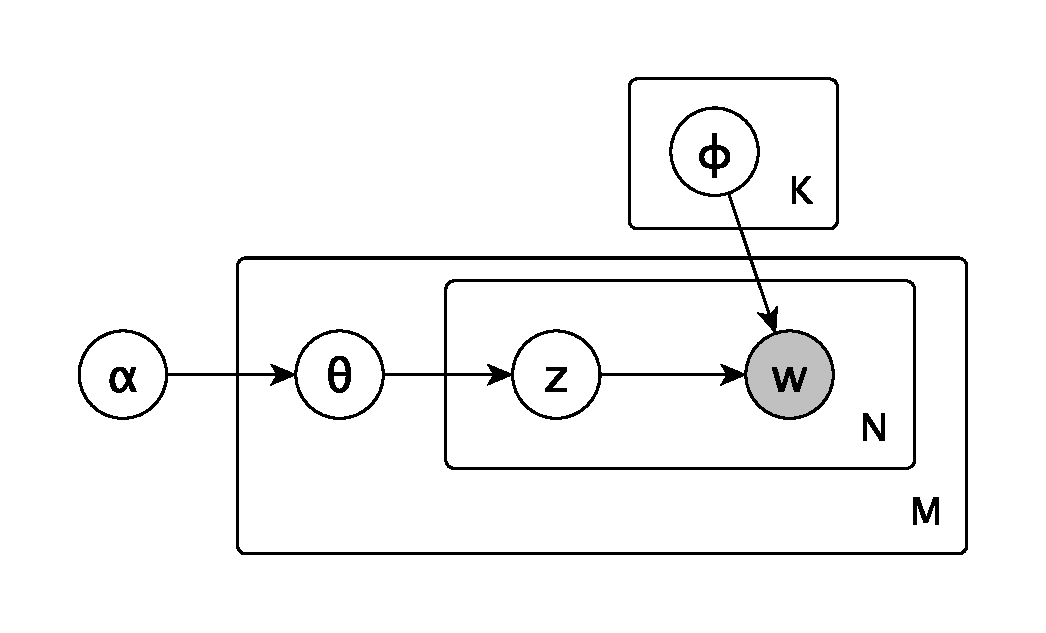
\includegraphics[scale=0.7]{figures/lda-generative-process.eps}
\caption{Diagram of the LDA model.}\label{fig:lda_gen_process}
\end{figure}

The generation of a corpus is done with the following steps~\cite{crain2012dimensionality, blei2003latent}:

\begin{itemize}
    \item \textbf{Draw a distribution over the words for each topic.}
        A sample $\phi_i$ is drawn from a symmetric Dirichlet distribution with parameter $\beta$. 
        This sample represents the distribution of terms for the topic $i$.

        \begin{equation}
            \Phi_i \sim Dir(\beta)
        \end{equation}

        \begin{equation}
            p(\Phi_i | \beta) = \frac{\Gamma(V\beta)}{{\Gamma(\beta)}^V} \prod^V_{v=1}\phi^{\beta-1}_{iv}
        \end{equation}

        Here, $\Gamma$ is the gamma function.

    \item \textbf{Draw a distribution over the topics for each document.}
        A sample $\theta_d$ is drawn from a Dirichlet distribution with parameters $\alpha$.
        This sample represents the distribution of topics for document $d$.

        \begin{equation}
            \Theta_d \sim Dir(\alpha)
        \end{equation}

        \begin{equation}
            p(\Theta_d | \alpha) = \frac{\Gamma(\sum^K_{i=1}\alpha_i)}{\prod_{i=1}^K\Gamma(\alpha_i)}\prod_{i=1}^K\theta_{di}^{\alpha_i-1}
        \end{equation}

    \item For each token with index n:

        \begin{itemize}
            \item \textbf{Draw a topic assignment $z_{dn}$ for the token index $n$.} 
                $z_{dn}$ is drawn from the distribution over topics for each document. 
                That is, $z_{dn}$ is drawn from a multinomial distribution using $\theta_d$ as a parameter.

                \begin{equation}
                    z_{dn} \sim Multinomial(\Theta_d)
                \end{equation}

                \begin{equation}
                    p(z_{dn} = i | \Theta_d) = \theta_{di}
                \end{equation}

            \item \textbf{Draw a token $w_{dn}$.}
                The token $w_{dn}$ is drawn from the topic distribution assigned to the index $n$.
                That is, $w_{dn}$ is drawn from a multinomial with parameter $\phi_{z_{dn}}$.

                \begin{equation}
                    w_{dn} \sim Multinomial(\Phi_{z_{dn}})
                \end{equation}

                \begin{equation}
                    p(w_{dn}=v|z_{dn}=i,\Phi_i) = \phi_{iv}
                \end{equation}

        \end{itemize}

\end{itemize}

The LDA model identifies topics from different terms that occur together.
Consider the case where an LDA model has been used to learn a number of topics.
Two terms that frequently occur together are then likely to be in the same topic.
So, if the same word has been used to express different thoughts, and the word has the same probability in two topics, the words that it co-occurs with can be used to differentiate between the different thoughts.

The task of learning the LDA model is a Bayesian Inference problem.
We have several variables that we cannot observe: the word distribution for the topics ($\phi_i$), the topic assignments for the tokens ($z$), and the topic distribution for the documents ($\theta_d$).
The only observed variables are the words in the document.
We have to approximate the posterior distribution using some sampling method, since it cannot be inferred automatically~\cite{blei2003latent}.

There exist a few algorithms that can be used to learn topics for the LDA model. 
Two of these that has shown to be able to extract useful topics from text are \textit{collapsed Gibbs sampling}~\cite{griffiths2004finding} and \textit{variational Bayes}~\cite{blei2003latent}.  
In collapsed Gibbs sampling, $\theta$ and $\phi$ are marginalized out.
It works by repeatedly sampling the topic assignment $z_{dn}$ for each token, conditioned on the assignments for the other tokens.
Variational Bayes works by using simpler single-variable models to approximate the LDA\@. 
As a consequence, it disregards any dependencies between the variables.
This is the approach used in the original LDA paper~\cite{blei2003latent}.

\subsubsection{Collapsed Gibbs}

% TODO: Write section on collapsed Gibbs
\textit{To be written}

\subsection{Text Clustering}

Cluster analysis is commonly defined as finding groups in a given dataset.
The members of these groups are determined to be similar by a similarity measure~\cite{kaufman2009finding, aggarwal2012survey}.
Since text data is sparse, but yet have a very high dimensionality.
With one dimension per term in the dictionary, it is not uncommon with dimensions in the order of $10^5$.
For this reason, some of the more naive clustering algorithms does not work as well for text data~\cite{aggarwal2012survey}.

In distance-based clustering, a similarity function is used to measure the closeness between two text documents.
For the purpose of measuring the similarity between text objects, the cosine similarity function is most commonly used~\cite{aggarwal2012survey}.
Two different approaches to distance-based clustering are distance-based partitioning, and agglomerative hierarchical clustering.
%For distance-based clustering k-means and k-medoid are two the frequently used algorithms.
%When it comes to text data, k-means is preferred since k-medoid does not work as well for sparse data, and requires more iterations to converge~\cite{aggarwal2012survey}.

\subsubsection{K-means Clustering}

When using the k-means clustering algorithm, the clusters are based upon an initial set of k representatives.
A simple approach to k-means clustering can be seen as:

\begin{enumerate}
    \item Select K seeds from the original dataset
    \item \label{enum:k-means-step-2} Assign the rest of the documents to one of these seeds, based how how similar they are by the similarity function
    \item \label{enum:k-means-step-3} Before each new iteration, select a new centroid for each cluster. This should be the point that is the best central point for the cluster.
    \item Repeat step \ref{enum:k-means-step-2} and \ref{enum:k-means-step-3} until convergence.
\end{enumerate}

A visualization of this can be seen in Figure~\ref{fig:kmeans-iterations}.
One advantage that K-means has over K-medoid is that it requires a small number of iterations, especially compared to K-medoid~\cite{aggarwal2012survey, schutze1997projections}.
However, K-means is rather sensitive to the selection of initial seeds.
One approach is to just select them randomly, or selecting them based on the result of another lightweight clustering method.
A frequently used method is k-means++, that has been shown to improve both the speed and accuracy of k-means clustering~\cite{arthur2007k}.

\begin{figure}[h!]
    \centering
    \thirdsubfig{kmeans-init}{Initial seeds}
    \thirdsubfig{kmeans-iter1}{Iteration 1}
    \newline
    \thirdsubfig{kmeans-init2}{Centroids after iteration 1}
    \thirdsubfig{kmeans-iter2}{Iteration 2}
    \thirdsubfig{kmeans-init3}{Centroids after iteration 2}
    \caption{(a) to (e) shows iterations of K-means until convergence.
        In (e) it can be seen that the new centroids capture the same documents as the previous iteration, and we have converged.}
    \label{fig:kmeans-iterations}
\end{figure}

\subsection{Word Embeddings with Word2Vec}

\textit{To be written}

\section{Text Classification}

Text classification is a widely studied field within Computer Science.
It is an important problem in supervised machine learning, and it is the task of assigning one or more classes to a given text document~\cite{aggarwal2012surveyclass}.
The problem is mainly approached with supervised machine learning.
That is, with a dataset that consists of a collection of text documents, where each document has one or more classes assigned to it. % TODO: QUOTE BISHOP
With the help of these labels, a classification model is fitted to the data.
The goal of this is for the model to be able to correctly assign a class to a a previously unseen text document.
Some of these classification models can also produce a probability of a document being of a certain class.
Other models are based on the concept of a margin that separates the classes, and the distance between a data point and a margin can be used to indicate how certain the model is of the assigned label~\cite{tong2001support}.
Example of use cases for text classification is categorization of news articles, document retrieval and email filtering.
There exists several different models for classifying text.
Decision trees, neural networks and Support Vector Machines (SVM) are some have been previously applied to the text domain with successful results~\cite{aggarwal2012survey}.
In this thesis, SVM are the main focus, since they have been studied extensively in the context of active learning. %TODO: CITE ALL OF THE SUPPORT VECTOR MACHINE ACTIVE LEARNING PAPERS

\subsection{Support Vector Machines}

SVMs work by implicitly map the training data to a feature space~\cite{bishop2006pattern}.
The goal is that the data should be linearly separable in the feature space, even if it is not in the input space.
In the case of binary classification, a point is classified by the linear model:

\begin{equation}
    y(x) = w^T \phi(x) + b
\end{equation}

The sign of $y(x)$ determines the label assigned to x.

SVMs work by trying to find the hyperplane that maximizes the margin.
That is, the distance between any point and the decision boundary should be as large as possible.
The hyperplane that gives us the maximum margin can be found by:

\begin{equation}
    \arg\min_{w,b}\frac{1}{2}||w||^2
\end{equation}

In order to allow for better generalization, and for data that isn't completely linearly separable, SVMs make use of slack variables $\xi_n$ to penalize points that are close to the decision boundary~\cite{bishop2006pattern}.
A parameter $C>0$ controls how much effect the slack variables will have.
The equation with the slack variables becomes:

\begin{equation}
    \arg\min_{w,b}\frac{1}{2}||w||^2 + C \sum_n\xi_n.
\end{equation}

A smaller $C$-value allows more points to be misclassified, in order to achieve better generalization.

\subsection{Multi-Label Classification}\label{subsec:multi-label-classification}

Multi-label classification is the type of text classification where one instance can be associated with multiple labels.
It is a generalized version of the multi-class classification problem, where you have more than 2 labels, but each document is only assigned one~\cite{tsoumakas2006multi}.

A common way of solving multi-label classification problems is the Binary Relevance method~\cite{read2011classifier, boutell2004learning, luaces2012binary}.
It is a way of transforming the multi-label classification problem into several different binary ones.
With Binary Relevance you fit one classification model per label in your data.
Each of these classifiers are then predicting whether or not the document is associated with the corresponding label or not.

\section{Active Learning}\label{sec:active-learning}

Conventional machine learning systems use a set of available data to find a hypothesis that can explain the patterns.
The purpose of active learning is to allow a system to \textit{select} the data that it wants labeled, and therefore the data it wants to be trained on~\cite{settles2012active}.
An active learning system samples a document to be labeled from a pool of unlabeled data, and then queries an oracle (often a human annotator) to get the label for that document.
By being able to decide what data to to label and use, the goal is that the system can achieve better results, and that the data will be of higher quality.
A model of the active learning system can be seen in Figure~\ref{fig:active-learning-model}.
\begin{figure}[!ht]
    \centering
    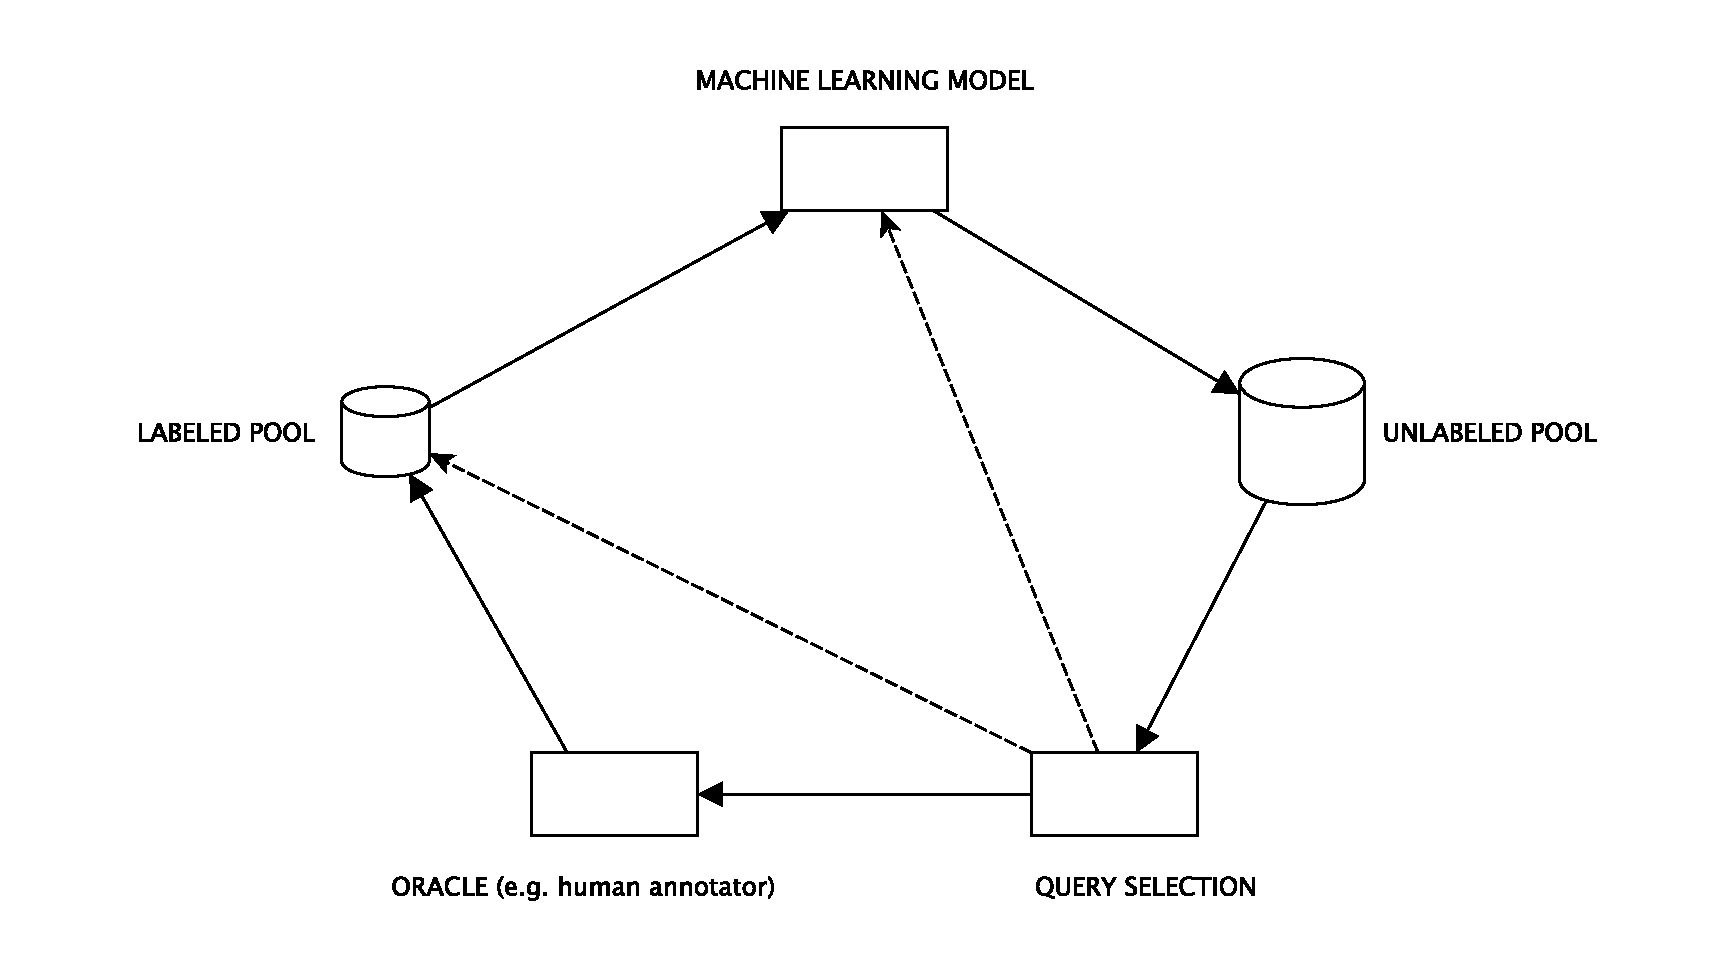
\includegraphics[scale=0.5]{figures/active-learning-model.eps}
    \caption{An overview of an active learning system}
    \label{fig:active-learning-model}
\end{figure}

In several different domains, data is readily available and easy to come by.
But even if the data is abundant, labels for the data is often harder and more expensive to come by~\cite{settles2012active}, especially when it comes to multi-label problems.

The next section will describe different ways to access the documents in active learning systems, followed by some theory of how the samples relate to the hypothesis space.
After that some concrete methods for selecting the samples to queried are described and compared.

\subsection{Pool-Based Sampling}

The main focus is how to select the samples to be labeled.
There are different sampling methods in use, and which one is more appropriate depends on how the data can be accessed.
Pool-based sampling is motivated by the assumption that there exists a large ready pool of data, where only a small portion is labeled~\cite{lewis1994sequential, settles2012active}.
The samples to be labeled is then selecting by evaluating the entire pool of unlabeled data, and select the most appropriate one based on a defined utility measure.
If the entire pool is large, a subset could be used instead.
For applied active learning, pool-based sampling seems to be the most popular choice, but there are some alternatives that have been used in theoretical settings such as stream-based selective sampling.
The difference between stream-based selective sampling and pool-based sampling is the individuality of the decisions in stream-based selective sampling, where you draw one sample at a time from an input source and make the decision whether or not to query a label for it.
For text applications, where a set of data is often readily available, pool-based sampling is often the more appropriate option since you can consider the entire dataset.
Pool-based is therefor the sampling technique that will be considered in this paper.

\subsection{Searching the Hypothesis Space}

In machine learning hypothesis is a specific configuration of a model, the purpose of which is to predict outputs on new instances of data by generalizing the training data.
One hypothesis can, for example, be an SVM model with specific values for the parameters.
The set of all possible hypothesis that we are working with the \textit{hypothesis space}.
Following the SVM example, the hypothesis space would be the set of SVM's with the different values that are possible for the parameters.
The hypothesis space is defined as:
% TODO: Big brackets
\begin{equation}
    \begin{aligned}
        \mathcal{H} = \Bigg \{ f | f(x) = \frac{w * \phi(x)}{|w|} \Bigg \}\\
        \text{where~$w \in \mathcal{W}$ and $\mathcal{W}$ is our parameter space}
    \end{aligned}
\end{equation}

The version space the subset of the hypothesis space
The subset of the hypothesis space that in the feature space separates the data is called the version space, which is defined as:

\begin{equation}\label{eq:version-space}
    \mathcal{V} = \Bigg \{ f \in \mathcal{H} | y_i f(x_i) > 0 \forall i \in \{i \dots n\} \Bigg \}
\end{equation}

So the version space therefore represents the different hypothesis that make correct predictions on the training data.
Under the assumption that one of the hypothesis can fully separate the data, the version space shrinks when more labeled data is acquired.
So for new labeled instances the hypotheses in the version space will give better predictions for the training data.
Based on this, an active learning algorithm should aim to reduce the size of the version space with each new sample, optimally make it half the size in each iteration.

There exists a useful relationship between the feature space $\mathcal{F}$ and the hypothesis space $\mathcal{H}$ called the \textit{version space duality}~\cite{tong2001support, vapnik1998statistical}.
It states that hyperplanes in the hypothesis corresponds to points in the feature space, and the other way around.
So by selecting points to be labeled, constraints can be enforced on the hypothesis that form the version space.

One approach to this is called that has shown to be successful is \textit{Uncertainty Sampling}~\cite{settles2012active}.
The idea behind SVM is to find a hyperplane that separates two classes in a binary classification with the maximum margin.
Out of the different hyperplanes in the hypothesis space, the version space contains those that can successfully separate the data.
We want to select the points in the feature space that will reduce the amount of the valid hypotheses the most.
Since SVMs tries to find the support vectors that maximizes the decision boundary in the feature space, separating the two classes.
Considering this in $\mathcal{H}$, it will be analogous to the hypothesis in the center of the hypothesis space encompassed constraints set by the labeled points.
What Uncertainty Sampling is predicting the values for the unlabeled points, and then choose the one that it is most uncertain about, the one closest to the decision boundary, to be labeled.
Based on the version space duality, it is a good approximation for dividing the version space in two.

\subsection{Binary Version Space Minimization}\label{subsec:binmin}

Binary Minimization is a generalization of uncertainty sampling, to make it work with multi-label data.
The approach taken is to decompose the multi-label problem to several binary one-vs-rest tasks, like discussed in~\ref{subsec:multi-label-classification}.
The unlabeled point that is chosen for labeling is then the one with the smallest SVM margin across all the binary classification tasks.
By doing this, it does not incorporate the multiple labels into the decision process, but treats all classes individually and equally. 

\subsection{Maximum Loss Reduction with Maximum Confidence}\label{subsec:mmc}

Maximum Los Reduction with Maximum Confidence(MMC) was developed by Yang et al~\cite{yang2009effective}.
The goal of the technique is to find the samples that will reduce the expected model loss the most, and select this sample for labeling.
These are the basic notations that will be used when explaining the MMC approach:
\begin{itemize}
    \item The labeled dataset: $D_L$.
    \item The unlabeled dataset: $D_U$.
    \item Possible query set: $D_S$.
    \item Optimal query set: $D^*_S$.
    \item The classification function that is trained on dataset $D_L$: $f_{D_L}$.
    \item A data point: $x$, and its label: $y$.
    \item The loss of on data point $x$: $L(f_{D_l}(x))$.
    \item The expected loss of the model: $\widehat{\sigma_{D_L}}$.
\end{itemize}

The expected model loss that MMC is trying to reduce can be defined as follows~\cite{yang2009effective}:
\begin{equation}
    \widehat{\sigma_{D_L}} = \int_x \bigg ( \sum_{x \in Y} L(f_{D_L})P(y|x) \bigg ) P(x)dx
\end{equation}

It is hard to estimate $P(x)$, so it is instead measured over all the samples in $D_U$.
This results in another estimate:
\begin{equation}
    \widehat{\sigma_{D_L}} = \frac{1}{|D_U|} \sum_{x \in D_U} \sum_{y \in Y} L(f_{D_L})P(y|x)
\end{equation}

After a set of data points $D_S$ has been labeled, the new dataset $D'_L=D_L + D_S$ is obtained.
Under the assumption that any $x \in D_U - D_S$ has an equal effect on a model trained on the datasets $D_L$ and $D'_L$, we get the following equation for the reduction of the expected loss~\cite{yang2009effective}:

\begin{equation}
    D^*_S = \arg\max_{D_S}(\widehat{\sigma_{D_L}} - \widehat{\sigma_{D'_L}}) = \arg\max_{D_S} \big ( \sum_{x \in D_S} \sum_{y \in Y} (L(f_{D_L}) - L(f_{D'_L})) P(y|x) \big )
\end{equation}

In their paper, Yang et al\@. considers the process of finding the greatest reduction in two steps: finding a good estimate for the conditional probability $p(y|x)$, and finding a way to assess the loss reduction of a multi-label classifier.

It is unfeasible for a query strategy to provide a an estimation for all possible label combinations.
If there are $n$ different labels, there will be $2^n$ different label combinations.
In order to estimate the conditional probability $p(y|x)$, MMC uses an approach that first estimates the number of labels for a given data point, and then uses that estimate to select the most probable labels.
Consider the case where a data point has $m$ labels.
Since we can obtain the probability from our classification model for each label, we can sort them in descending order.
The first $m$ labels are then likely to have a high probability, while the rest a rather low probability.

Yang et al\@.~\cite{yang2009effective} describes the process of estimating the number of labels as follows:
\begin{enumerate}
    \item Use the classification model to obtain the probabilities for each label for all the data samples.
    \item For each data sample, sort and normalize the probabilities for all the labels.
    \item Using the labeled dataset, train a logistic regression classifier with the sorted and normalized probabilities as features, and the number of labels as target.
    \item With the trained logistic regression model, predict the number of labels for the samples in the unlabeled pool.
\end{enumerate}

After obtaining the predicted number of labels $m$ for a sample $x$, the estimate for $p(y|x)$, denoted $\hat{y}$, is then obtained by selecting $m$ the most probable labels based on the original classification models output.

The only task that's left is now to estimate the loss for the multi-label classifier.
By using the model where there are $k$ different binary classifiers for a problem with $k$ labels, the model loss can be calculated by adding the loss for the different binary classifiers like:

\begin{equation}
    L(f) = \sum_{i = 1}^k L(f^i)
\end{equation}

where the loss of a single binary classifier is denoted as $L(f^i)$.
With this definition, it only remains to define the measure of loss on a single binary classifier.
The measurement that is used by MMC is to estimate the model loss by the size of the version space of the SVM~\cite{tong2001support, yang2009effective}.
The version space's size can be computed with Equation~\ref{eq:version-space}.
However, computing this for each possible label set is expensive.
By using the heuristic from~\cite{tong2001active}, an approximation of the version space with the added label can be obtained from the current SVM classifiers' margin.
The reduction rate after adding a the data point $(x, y^i)$, where $y^i \in {-1, 1}$, can be expressed as follows~\cite{yang2009effective, tong2001active}:

\begin{equation}\label{eq:reduction-rate}
    \frac{L(f^i_{D_L+(x, y^i)})}{L(f^i_{D_L})} \approx \frac{V^i_{D_L + (x, y^i)}}{V^i_{D_L}} \approx \frac{1 + y^i f^i_{D_L}(x)}{2}
\end{equation}

$L(f^i_{D_L})$ does not involve the sample selected for labeling, so by writing the loss reduction as:
\begin{equation}
    \begin{split}
        L(f_{D_L}) - L(f_{D'_L}) = \sum_{i=1}^k\big ( L(f^i_{D_L}) - L(F^i_{D'_L}) \big )\\
        = \sum_{i=1}^k\big ( L(f^i_{D_L}) \dot (1 - \frac{L(F^i_{D'_L})}{L(F^i_{D_L})}) \big )
    \end{split}
\end{equation}

it can be seen that focusing on the reduction rate is sufficient.
By incorporating the result from Equation~\ref{eq:reduction-rate}, the following approximation for the reduction rate is obtained:

\begin{equation}
    \sum_{i=1}^k\big ( \frac{1 - y^if^i_{D_L}(x)}{2} \big )
\end{equation}

The only thing that remains is now to combine the estimation of $p(x|y)$ with the estimate for loss reduction.
The resulting equation, called maximum loss reduction with maximal confidence, is~\cite{yang2009effective}:

\begin{equation}
    D^*_S = \arg \max_{D_S} \big ( \sum_{x \in D_S} \sum_{i=1}^k (\frac{1 - \hat{y}^if^i_{D_L}(x)}{2}) \big )
\end{equation}

\subsection{Adaptive Active Learning}\label{subsec:adaptive-active-learning}

In their paper, Li et al\@.~\cite{li2013active} presents two approaches to active learning:
\begin{itemize}
    \item Max-Margin Uncertainty Sampling
    \item Label Cardinality Inconsistency 
\end{itemize}
These two techniques are then combined in a weighted fashion into what they call Adaptive Active Learning.

\subsubsection{Max-Margin Uncertainty Sampling}

The idea behind \textit{Max-Margin Uncertainty Sampling} comes from the observation that multi-label classification prediction is mainly about separating the positive labels from the negative labels~\cite{li2013active}.
That is, separating the labels gets assigned to an instance and the ones that does not.
In order to model the uncertainty of the prediction of the prediction on a datapoint, Li et al\@. suggest the usage of a global separation margin to separate the negative labels from the positive.

The positive labels for a data point $x$ is defined as those where $sign(f'_{D_L}(x))$ is positive.
The separation margin is defined as:
\begin{equation}
    \begin{split}
        sep\_margin(x) = \min_{i \in \hat{y}^+}f'_{D_L}(x) - \min_{i \in \hat{y}^-}f'_{D_L}(x) \\
        = \min_{i \in \hat{y}^+}|f'_{D_L}(x)| + \min_{i \in \hat{y}^-}|f'_{D_L}(x)|
    \end{split}
\end{equation}
where $\hat{y}^+$ denotes the set of predicted labels that are positive on the instance, and the $\hat{y}^-$ denotes the negative ones.

The data point that the model is the most uncertain about is then the one with the smallest margin.
Li et al\@. define their global measure, max-margin prediction uncertainty, as:
\begin{equation}
    u(X) = \frac{1}{sep\_margin(X)}
\end{equation}

\subsubsection{Label Cardinality Inconsistency}

\textit{Label Cardinality Inconsistency} is based on that the underlying distribution is the same for the labeled and unlabeled data.
In a multi-label dataset, the \textit{label cardinality} is defined as the average number of labels assigned to each class~\cite{tsoumakas2006multi}.
The selection strategy that Li et al\@. based on this measures the Euclidean distance between the number of assigned predicted labels on $x$, and the label cardinality of the labeled data:

\begin{equation}
    c(x) = \bigg \lVert \sum_{i \in \hat{y}^+} 1 - \frac{1}{N_L} \sum_{y \in Y_L} \sum_{i \in y^+} 1 \bigg \rVert_2
\end{equation}

where $N_L$ is the number of labeled samples, $Y_L$ are the labels for those samples, and $y^+$ are the positive labels in $y$.

\subsubsection{Integration - Adaptive Active Learning}

Since \textit{max-margin uncertainty sampling} and \textit{label cardinality inconsistency} complement each other, an integration method is used:
\begin{equation}\label{eq:approx-generalization-error}
    q(x, \beta) = u(x)^\beta \cdot c(x)^{1-\beta}
\end{equation}

where $\beta$ is a parameter controlling the weight put on the two measures.
This parameter is chosen by in each iteration evaluating a discrete set of values, for example $\{0, 0.1, 0.2, \dots, 1\}$.
Then selecting $\beta$ based on the most informative sample amongst the .
Equation~\ref{eq:approx-generalization-error} shows the \textit{approximate generalization error}, which is used to select the sample.
\begin{equation}
    \epsilon(x) = \sum_{x \in D_U} \max_{i \in f(x)^+}(1-f^i(x)) + \max_{i \in f(x)^-}(1+f^i(x))
\end{equation}

where $f(x)^+$ and $f(x)^-$ are the predicted positive labels, and negative labels, respectively.
So, the sample is then selected by:
\begin{equation}
    x^* = \arg \min_{x \in D_U} \epsilon(x)
\end{equation}

\section{Evaluation Metrics}

For classification of information retrieval systems the typical evaluation metrics to use are \textit{precision}, \textit{recall} and \textit{recall}~\cite{jiang2012information}.
We define the following metrics in terms of \textit{true positives}, \textit{false positives}, \textit{true negatives} and \textit{false negatives}.
How they are defined can be seen in table~\ref{tab:conf-matr}.
Data points that are correctly classified are then either \textit{true positives} or \textit{true negatives}.

\begin{table}[!ht]
    \begin{center}
        \begin{tabular}{c c c}
            & Correct P & Correct N \\
            \toprule
            Predicted P & True Positive & False Positive \\
            Predicted N & False Negative & True Negative \\
        \end{tabular}
    \end{center}
    \caption{Confusion matrix for explaining true positives, false positives, true negatives and false negatives}\label{tab:conf-matr}
\end{table}

Precision is the percentage of the results found by the system that are correct~\cite{tjong2003introduction}.
Recall is the percentage of correct results in the dataset that are found by the system.
Precision and recall are defined as follows by Van Rijsbergen~\cite{rijsenbergen1979information}:

\begin{equation}
    Precision = \frac{tp}{tp+fp}
\end{equation}

\begin{equation}
    Recall = \frac{tp}{tp+fn}
\end{equation}

F-score is the harmonic mean between recall and precision, and is defined as~\cite{tjong2003introduction}:

\begin{equation}
    F = \frac{2*precision*recall}{precision+recall}
\end{equation}

Another metric that is used for evaluation is \textit{accuracy}, which is defined as follows:

\begin{equation}
    Accuracy = \frac{tp+tn}{tp+tn+fp+fn}
\end{equation}

These metrics mainly work
\section{Related Work}

Using topic modeling for various clinical applications has been done before.
Topic modeling have been a popular approach for this purpose since clinical data often is in the form of free text.
The resulting topics can be interpreted by humans, which allow doctors to get more insight into the system.
Sarioglu et al\@.~\cite{sarioglu2013topic} to represent clinical reports with topic vectors in order to classify them.
Chan et al\@.~\cite{chan2013empirical} used topic models to analyze patient records and clinical reports from cancer patients.
In their paper, they found relationships between the content of the notes on the patients, with the data that was available on the patients' genetic mutations.
The interpretability of topics generated from an LDA model was studied on clinical reports by Arnold et al~\cite{arnold2016evaluating}.
They evaluated how interpretable topics were based on how many topics the model used.

Active learning has been researched in text classification with different approaches.
They can be seen as two categories: searching through the hypothesis space by using the uncertainty of a model, or by exploiting the structure of the data through clustering~\cite{dasgupta2008hierarchical}.

One of the common baselines for active learning is uncertainty sampling~\cite{lewis1994sequential}.
That simply queries the label for the data point the model is most uncertain about.
In~\cite{dasgupta2008hierarchical} hierarchical clustering is used in an active learning system.
The labels are queried from clusters where there is a lot of uncertainty when it comes to the majority label.
By pruning the tree of clusters while querying for labels the goal is to obtain a pruning where each node mostly contains one label.

In \cite{nguyen2004active} they also take advantage of a clustering to select the samples to be labeled in a two-class environment.
They take advantage of that the data points closest to the centroids are the most important ones, and that most data points in one cluster have the same label.
What this approach has in common with a lot of the current research is that it is treating single-label or binary classification problems, which cannot be directly applied to a multi-label scenario.

Research in~\cite{brinker2006active} is dealing with the multi-label problem.
That is the paper that developed the \textit{binary version space minimization} strategy that is described in section~\ref{subsec:binmin}.
The MMC strategy that is described in section~\ref{subsec:mmc}, and the adaptive active learning strategy in section~\ref{subsec:adaptive-active-learning} are also techniques for managing the multi-label problem.
For image classification, there has been some methods develop, for example ~\cite{li2004multilabel, qi2008two}.
In~\cite{li2004multilabel} the goal is to, after making predictions, selecting the sample with the biggest mean loss.
However experiments have shown that this is not as suitable for text classification~\cite{yang2009effective}.
In~\cite{qi2008two}, the approach is to use pairs of labels and samples to present to the annotator, and the aim is to minimize the Bayesian classification error.
Due to the fact that labeling for text classification is more time consuming than image classification, since you have to read an entire text, this approach is not suitable for text classification~\cite{yang2009effective}.

Active learning has been used to deal with the problem of imbalanced datasets before.
In a binary classification setting, Ertekin et al\@.~\cite{ertekin2007learning} used uncertainty sampling with SVMs to get a more balanced dataset.
In~\cite{attenberg2013class}, Attenberg et al\@. uses density based active learning to improve the class balance.
However, it does not attempt to apply this in a multi-label setting.